\section*{Problem 4}
\begin{align*}
	&\text{Multiplexing gain}\qquad\qquad G_{\mathrm{m}}=\lim_{\mathrm{SNR}\rightarrow\infty}\frac{R}{\ld\left(\mathrm{SNR}\right)}& \\
	&\text{Diversity gain}\quad\qquad\qquad C=\ld\left(1+\mathrm{SNR}\right)\quad\Rightarrow\quad C\overset{\mathrm{SNR}\rightarrow\infty}{\approx}\ld\left(\mathrm{SNR}\right)& \\
	&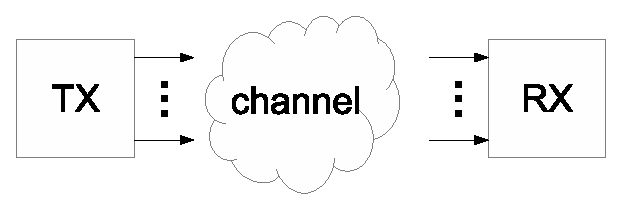
\includegraphics[width=0.7\textwidth]{MIMO_channel.eps}& \\
	&\text{Multiplexing gain $=$ number of parallel independent equivalent channels}& \\
	&\svd\left(H\right)\quad\rightarrow\quad\text{singular values of $H$: $\sigma_{i}^{2}$, $i\in\{1,2,\ldots,\rank\left(H\right)\}$}& \\
	&\rank\left(H\right)\quad\rightarrow\quad\text{number of singular values}& \\
	&H_{1}=
	\begin{bmatrix}
	1 & 1 & -1 \\
	-1 & 1 & 1 \\
	-1 & -1 & 1
	\end{bmatrix}\quad\rightarrow\quad\rank\left(H_{1}\right)=2& \\
	&\text{Matlab/Octave}\quad\rightarrow\quad\svd\left(H_{1}\right)=\mathbf{U}_{1}\mathbf{\Sigma}_{1}\mathbf{V}_{1}^{H}& \\
	&\qquad\mathbf{\Sigma}_{1}=
	\begin{bmatrix}
	2,56 & 0 & 0 \\
	0 & 1,56 & 0 \\
	0 & 0 & 0 
	\end{bmatrix}\quad\rightarrow\quad\text{$\sigma_{1}=2,56$, $\sigma_{2}=1,56$, $\sigma_{3}=0$ $\rightarrow$ useless}& \\
	&H_{2}=
	\begin{bmatrix}
	1 & -1 & -1 \\
	-1 & -1 & 1 \\
	1 & -1 & 1
	\end{bmatrix}\quad\rightarrow\quad\rank\left(H_{2}\right)=3\quad\rightarrow\quad\text{full rank}& \\
	&\svd\left(H_{1}\right)=\mathbf{U}_{2}\mathbf{\Sigma}_{2}\mathbf{V}_{2}^{H}& \\
	&\qquad\mathbf{\Sigma}_{2}=
	\begin{bmatrix}
	2 & 0 & 0 \\
	0 & 2 & 0 \\
	0 & 0 & 1 
	\end{bmatrix}\quad\rightarrow\quad\text{$\sigma_{1}=2$, $\sigma_{2}=2$, $\sigma_{3}=1$}& \\
\end{align*}